\documentclass[a4paper,12pt]{article}
\usepackage[utf8]{inputenc}
\usepackage[T1]{fontenc}
\usepackage[french]{babel}
\usepackage{amsmath, amssymb}
\usepackage{graphicx}
\usepackage{hyperref}
\usepackage{geometry}
\geometry{margin=2.5cm}

\title{Impact du cache sur la multiplication de matrices}
\author{
    Nathan Fontaine
    \\ 
    Hugo Viala
    \\ 
    Dardan Bytyqi
    \\
    }
\date{\today}

\begin{document}

\maketitle

\section{Introduction}

\subsection*{Contexte}
La multiplication de matrices est une opération fondamentale en calcul scientifique, utilisée dans de nombreux domaines tels que l'intelligence artificielle, la simulation numérique ou le traitement d'images. Les performances de cette opération dépendent fortement de l'architecture matérielle, notamment du processeur (CPU) et de la gestion du cache mémoire. Comprendre l'impact du cache sur l'efficacité de la multiplication de matrices permet d'optimiser les algorithmes et d'adapter les logiciels aux différentes plateformes matérielles.

\subsection*{Problématisation}
Comment le comportement du cache mémoire influence-t-il les performances de la multiplication de matrices?
Plus précisément, en quoi le choix de l'algorithme d'itération (ordre des boucles), 
la taille des matrices (\(N\)), le type de CPU et le système d'exploitation modifient-ils 
l'efficacité de l'utilisation du cache et donc les performances globales?

\subsection*{Hypothèses}
\begin{itemize}
    \item L'ordre d'itération des boucles (algorithmes ijk, jik, kij, etc.) a un impact significatif sur l'utilisation du cache et donc sur les performances.
    \item L'effet du cache varie selon la taille des matrices (\(N\)), avec des seuils où les performances chutent lorsque les données ne tiennent plus dans le cache.
    \item Les différences de CPU et de système d'exploitation influencent également l'efficacité du cache.
\end{itemize}

\subsection*{Plan du document}
Ce rapport est structuré comme suit: la section~2 décrit la méthodologie, 
incluant les notations, les algorithmes testés et le protocole expérimental. 
La section~3 présente et analyse les résultats obtenus. 
Enfin, la section~4 conclut et propose des perspectives d'amélioration.

\section{Méthodologie}

\subsection*{Notations}
\begin{itemize}
    \item \(N\) : taille des matrices carrées (\(N \times N\))
    \item \(t\) : temps d'exécution mesuré (en microsecondes)
    \item \texttt{algo} : nom de l'algorithme utilisé (ijk, jik, kij, etc.)
    \item FLOPS : nombre d'opérations flottantes par seconde
\end{itemize}

\subsection*{Description de la méthode}
Nous utilisons l'implémentations avec plusieurs variantes de la multiplication de matrices 
(\texttt{ijk}, \texttt{jik}, \texttt{kij}, etc.) dans le fichier \texttt{main.c}. 
Chaque algorithme diffère par l'ordre d'imbrication des boucles, 
ce qui influence l'accès mémoire et donc l'utilisation du cache. 
Un script Python automatise l'exécution des benchmarks pour différentes 
tailles de matrices et collecte les temps d'exécution dans un fichier CSV.

\subsection*{Protocole expérimental}
\begin{itemize}
    \item Compilation du code C sur différentes plateformes (Linux, Windows, Mac, ARM, AMD64).
    \item Exécution automatique des benchmarks via un script ou un notebook, sans intervention manuelle.
    \item Mesure du temps d'exécution pour chaque algorithme et chaque taille de matrice.
    \item Génération des résultats sous forme de fichiers CSV et de graphiques (FLOPS en fonction de \(N\)).
    \item L'environnement est reproductible grâce à un Dockerfile et une documentation détaillée.
\end{itemize}

\section{Résultats et discussion}

\subsection*{Résultats}
Les résultats sont présentés sous forme de graphiques montrant l'évolution des FLOPS en fonction de la taille \(N\) pour chaque algorithme. On observe des variations de performance selon l'ordre des boucles et des ruptures de pente lorsque la taille des matrices dépasse la capacité du cache.

\begin{figure}[h]
    \centering
    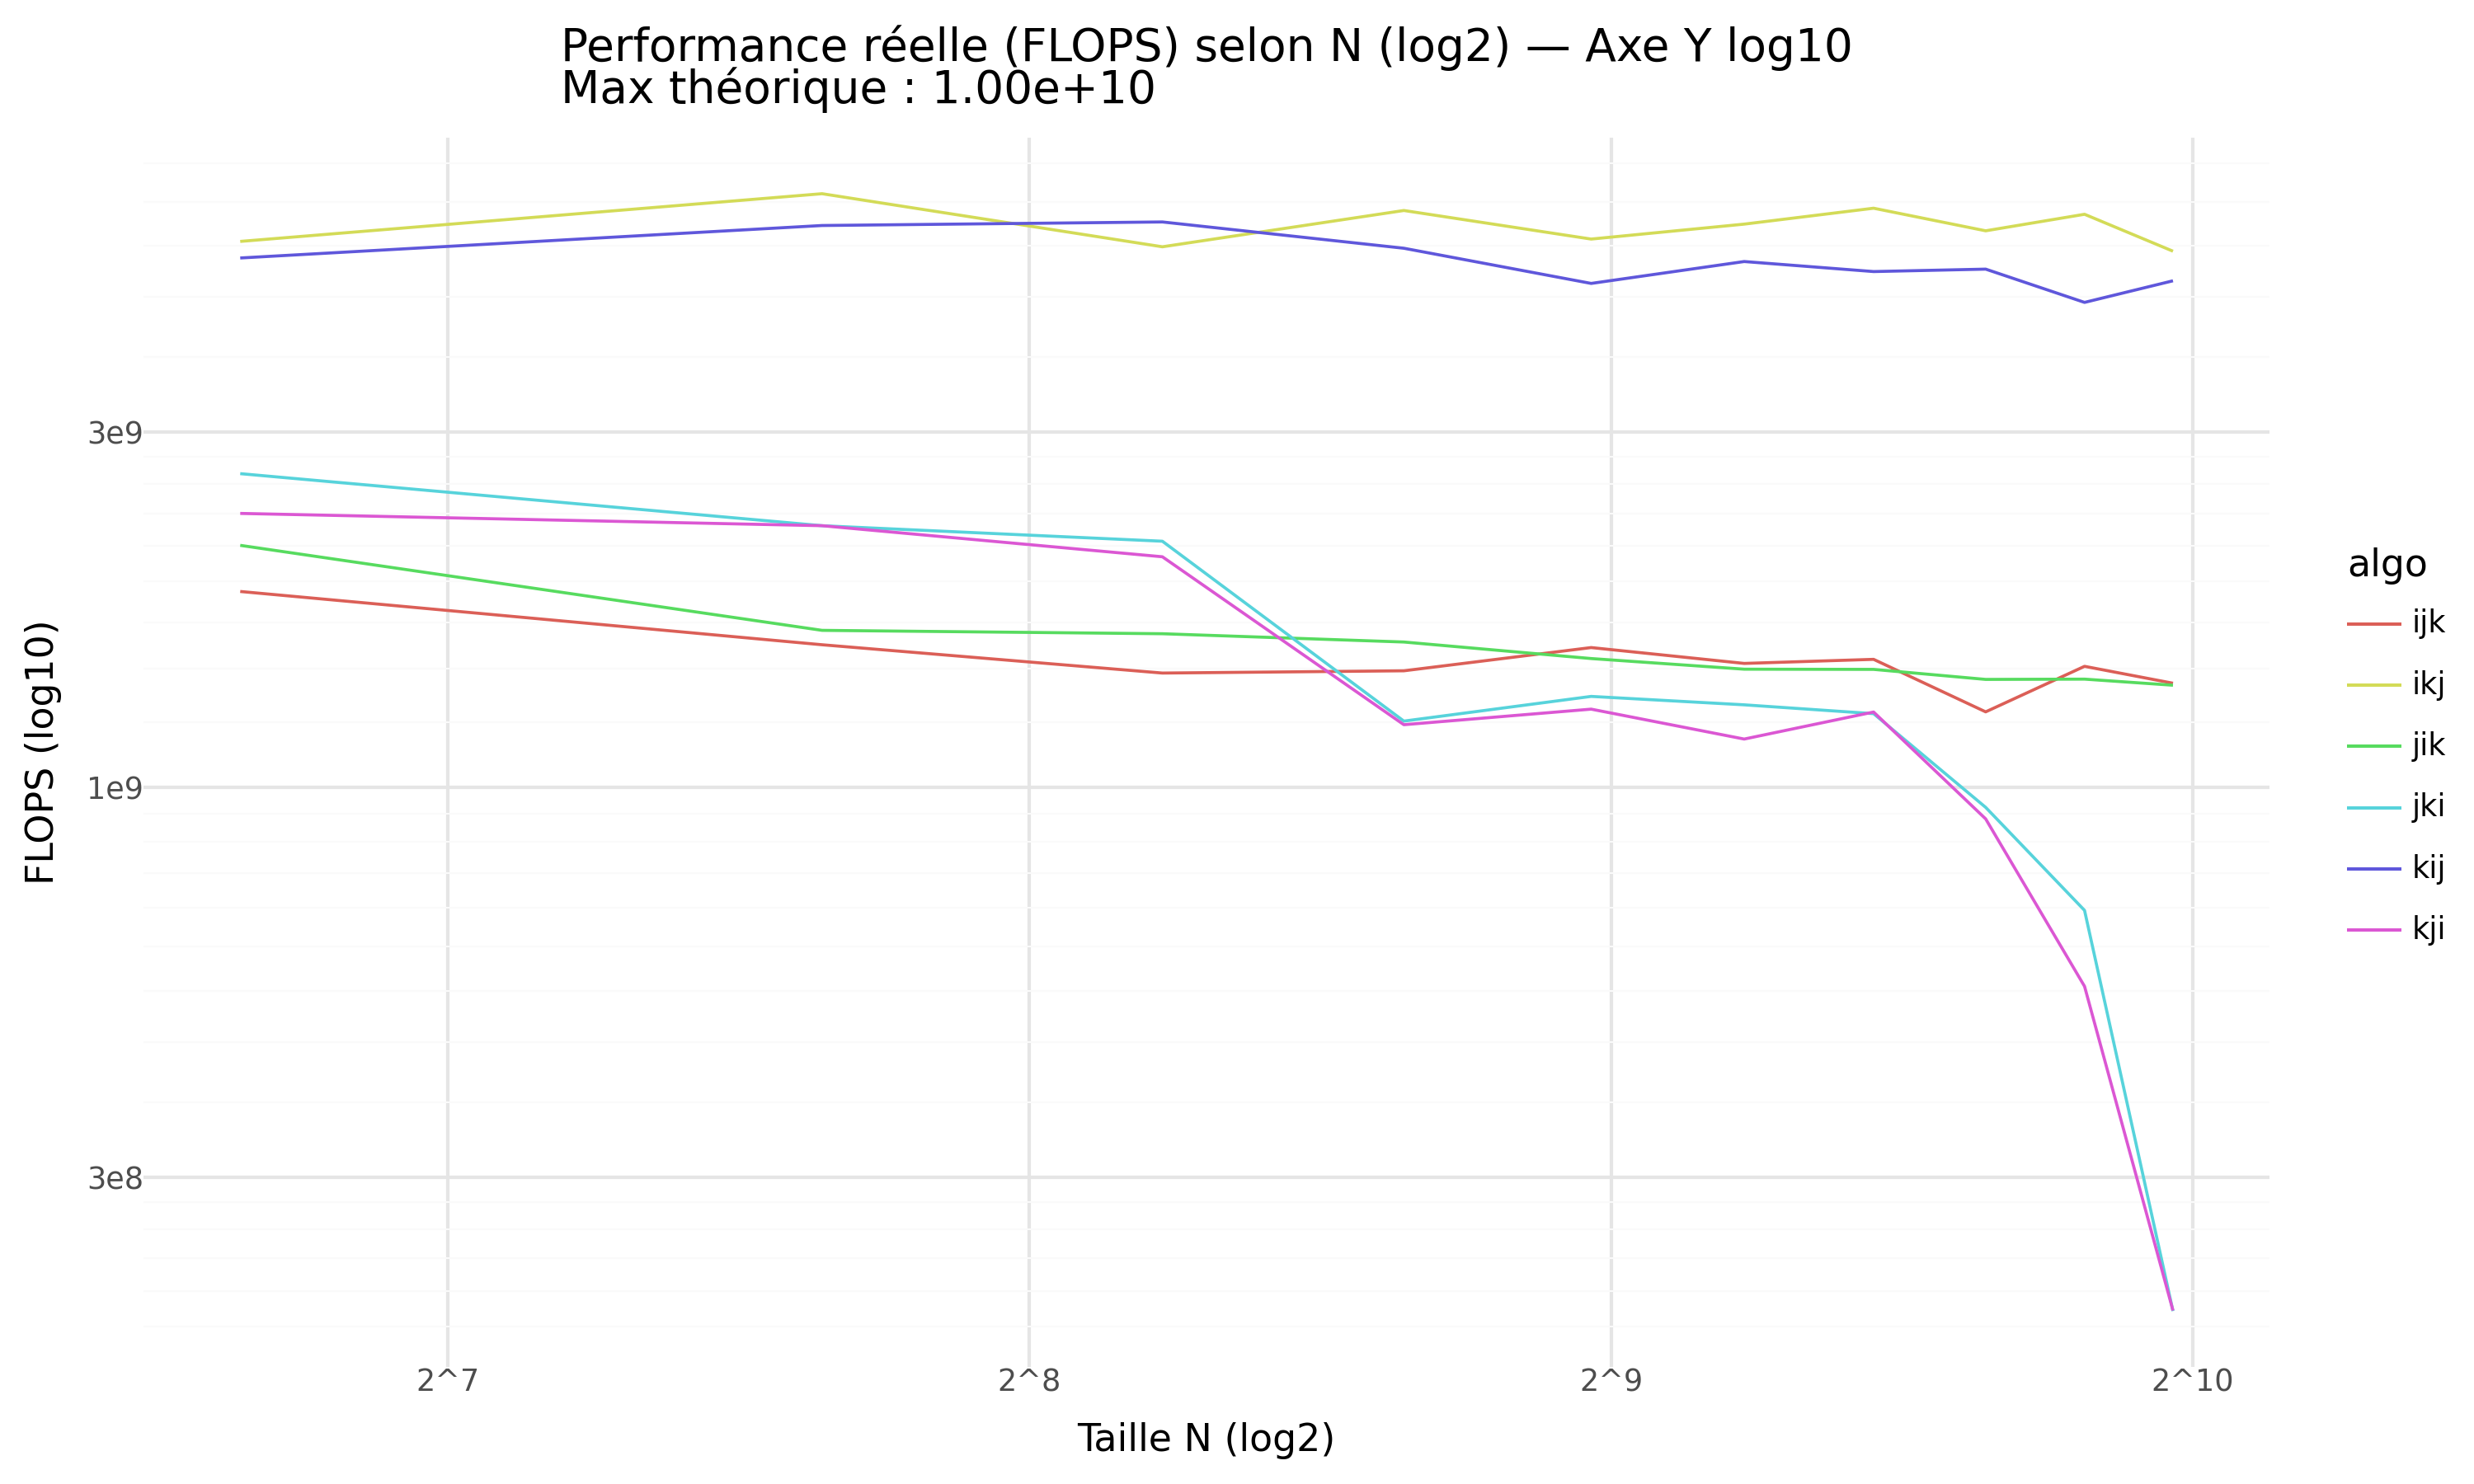
\includegraphics[width=1.2\textwidth]{../data/resultats_flops_plot.png}
    \caption{Performance réelle (FLOPS) selon \(N\) pour différents algorithmes}
\end{figure}

\subsection*{Discussion}
L'analyse des résultats montre que certains ordres de boucles exploitent mieux la localité mémoire, ce qui se traduit par de meilleures performances tant que les matrices tiennent dans le cache. Lorsque \(N\) augmente, les performances chutent brutalement, illustrant l'impact du cache. Les différences entre CPU et OS sont également notables, confirmant l'importance de l'architecture matérielle et logicielle.

\section{Conclusion}

Ce travail a permis de quantifier l'impact du cache sur la multiplication de matrices
en fonction de l'algorithme, de la taille des matrices, du CPU et du système d'exploitation. 
Les hypothèses de départ sont confirmées: l'ordre des boucles et la taille des matrices 
influencent fortement les performances via le cache. Pour aller plus loin, 
il serait intéressant de tester d'autres architectures, d'autres tailles de cache, 
ou d'optimiser encore les algorithmes.

\end{document}